\hypertarget{kdbtypes_8h}{}\section{kdbtypes.\+h File Reference}
\label{kdbtypes_8h}\index{kdbtypes.\+h@{kdbtypes.\+h}}


Elektra’s data types for C and C++11.  


{\ttfamily \#include \char`\"{}kdbconfig.\+h\char`\"{}}\newline
Include dependency graph for kdbtypes.\+h\+:
\nopagebreak
\begin{figure}[H]
\begin{center}
\leavevmode
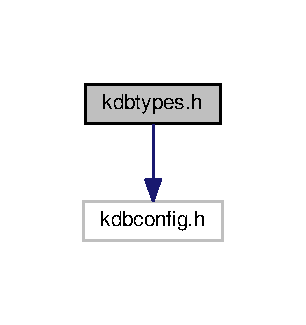
\includegraphics[width=147pt]{kdbtypes_8h__incl}
\end{center}
\end{figure}
This graph shows which files directly or indirectly include this file\+:
\nopagebreak
\begin{figure}[H]
\begin{center}
\leavevmode
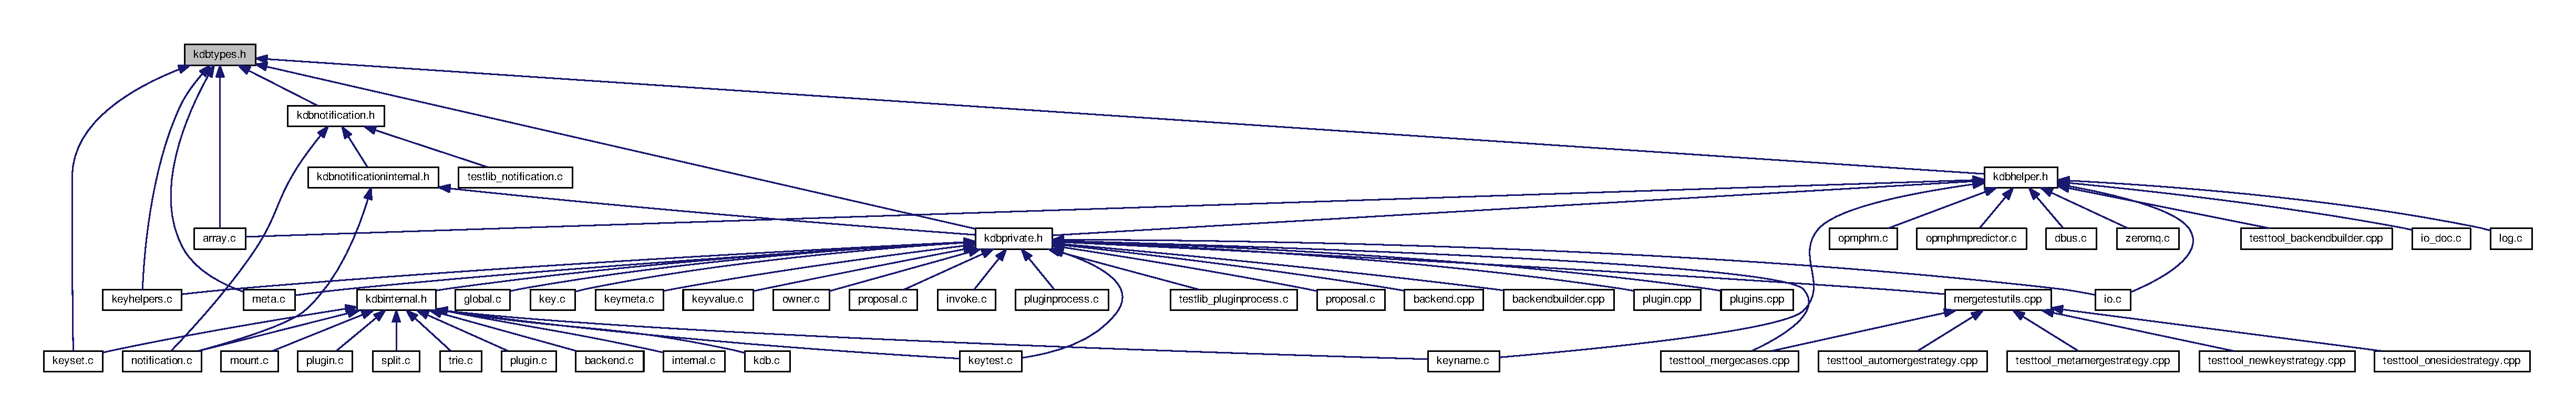
\includegraphics[width=350pt]{kdbtypes_8h__dep__incl}
\end{center}
\end{figure}


\subsection{Detailed Description}
Elektra’s data types for C and C++11. 

This header file defines portable Types used in Elektra for C and C++11.

They are not used within the A\+PI, but only for generated front ends see \char`\"{}kdb gen\char`\"{} how to use these types properly.

The C\+O\+R\+BA Type System is currently used.

See \char`\"{}\+O\+M\+G Language Mapping\char`\"{} if you want to map the types to another programming language.

This files defines mappings to C89, C++03 and C++11.

\begin{DoxyCopyright}{Copyright}
B\+SD License (see L\+I\+C\+E\+N\+S\+E.\+md or \href{https://www.libelektra.org}{\tt https\+://www.\+libelektra.\+org}) 
\end{DoxyCopyright}
